\documentclass[11pt]{article}

\usepackage[margin=1in]{geometry}
\usepackage[T1]{fontenc}
\usepackage{amsmath,amssymb}
\usepackage{graphicx}
\usepackage{booktabs}
\usepackage{tabularx}
\usepackage{array}
\usepackage{tikz}
\usetikzlibrary{arrows.meta,positioning,fit}
\usepackage[hidelinks]{hyperref}
\usepackage{microtype}
\usepackage{float}
\usepackage{placeins}

\begin{document}

\section{Background}

\subsection{Transformer Architecture}

The Transformer architecture, introduced by Vaswani et al.\ in
\textit{Attention Is All You Need}, established attention as the
principal mechanism for sequence modeling \cite{vaswani2017attention}.
Unlike recurrent architectures, the Transformer processes sequence
positions in parallel during training, enabling more efficient use of
accelerator hardware. Self-attention produces contextual representations
by allowing each token to aggregate information from other positions
in the sequence.

The original architecture comprises an encoder and a decoder, as
illustrated in Figure~\ref{fig:transformer}. Encoder layers contain
multi-head self-attention and position-wise feed-forward networks, with
residual connections and layer normalization surrounding each sublayer.
Decoder layers additionally employ masked self-attention and
cross-attention to encoder representations. The causal mask prevents
access to future tokens during autoregressive prediction. Positional
encodings supply information about token order, which the attention
operation alone does not explicitly represent
\cite{vaswani2017attention}.

\begin{figure}[htbp]
    \centering
    \resizebox{0.95\textwidth}{!}{%
    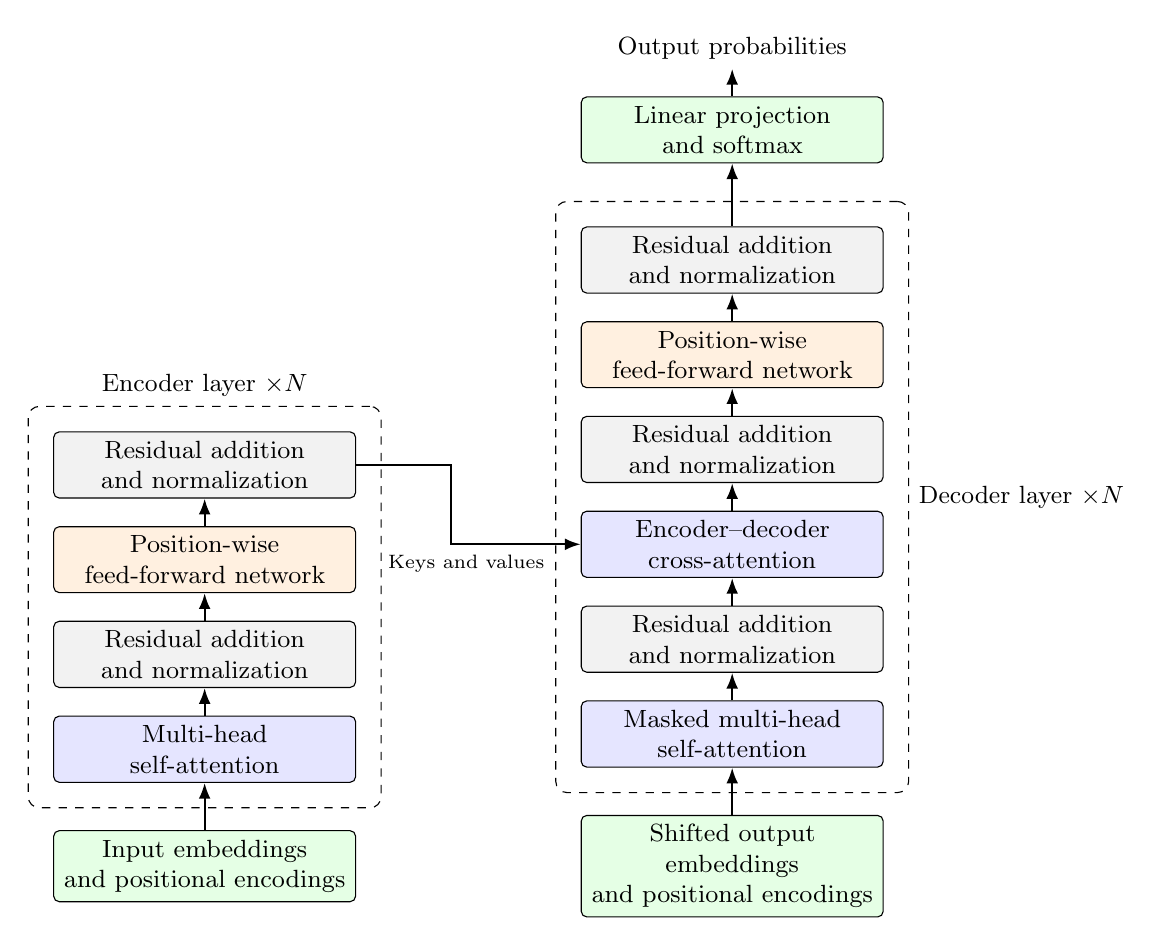
\begin{tikzpicture}[
        block/.style={
            draw,
            rounded corners=2pt,
            align=center,
            minimum width=3.8cm,
            minimum height=0.8cm,
            text width=3.6cm,
            font=\small
        },
        attention/.style={block, fill=blue!10},
        feedforward/.style={block, fill=orange!12},
        norm/.style={block, fill=gray!10},
        io/.style={block, fill=green!10},
        arrow/.style={-{Latex[length=2mm]}, thick},
        group/.style={
            draw,
            dashed,
            rounded corners,
            inner sep=9pt
        }
    ]

    % Encoder stack
    \node[io] (input) at (0,0)
        {Input embeddings\\and positional encodings};

    \node[attention, above=0.6cm of input] (encattn)
        {Multi-head\\self-attention};

    \node[norm, above=0.35cm of encattn] (encnormone)
        {Residual addition\\and normalization};

    \node[feedforward, above=0.35cm of encnormone] (encff)
        {Position-wise\\feed-forward network};

    \node[norm, above=0.35cm of encff] (encnormtwo)
        {Residual addition\\and normalization};

    % Decoder stack
    \node[io] (outputinput) at (6.7,0)
        {Shifted output embeddings\\and positional encodings};

    \node[attention, above=0.6cm of outputinput] (decattn)
        {Masked multi-head\\self-attention};

    \node[norm, above=0.35cm of decattn] (decnormone)
        {Residual addition\\and normalization};

    \node[attention, above=0.35cm of decnormone] (crossattn)
        {Encoder--decoder\\cross-attention};

    \node[norm, above=0.35cm of crossattn] (decnormtwo)
        {Residual addition\\and normalization};

    \node[feedforward, above=0.35cm of decnormtwo] (decff)
        {Position-wise\\feed-forward network};

    \node[norm, above=0.35cm of decff] (decnormthree)
        {Residual addition\\and normalization};

    \node[io, above=0.8cm of decnormthree] (projection)
        {Linear projection\\and softmax};

    \node[above=0.35cm of projection, font=\small] (probabilities)
        {Output probabilities};

    % Main data flow
    \draw[arrow] (input) -- (encattn);
    \draw[arrow] (encattn) -- (encnormone);
    \draw[arrow] (encnormone) -- (encff);
    \draw[arrow] (encff) -- (encnormtwo);

    \draw[arrow] (outputinput) -- (decattn);
    \draw[arrow] (decattn) -- (decnormone);
    \draw[arrow] (decnormone) -- (crossattn);
    \draw[arrow] (crossattn) -- (decnormtwo);
    \draw[arrow] (decnormtwo) -- (decff);
    \draw[arrow] (decff) -- (decnormthree);
    \draw[arrow] (decnormthree) -- (projection);
    \draw[arrow] (projection) -- (probabilities);

    % Encoder output supplies keys and values
    \draw[arrow]
        (encnormtwo.east) --
        ++(1.2,0) |-
        node[pos=0.56, below, font=\scriptsize]
        {Keys and values}
        (crossattn.west);

    % Repeated layer boundaries
    \node[
        group,
        fit=(encattn)(encnormtwo),
        label={[font=\small]above:Encoder layer $\times N$}
    ] {};

    \node[
        group,
        fit=(decattn)(decnormthree),
        label={[font=\small]right:Decoder layer $\times N$}
    ] {};

    \end{tikzpicture}%
    }
    \caption{
        Simplified encoder--decoder Transformer architecture.
        Each residual addition combines a sublayer output with its
        input. Encoder outputs provide keys and values to decoder
        cross-attention. Adapted conceptually from
        Vaswani et al.~\cite{vaswani2017attention}.
    }
    \label{fig:transformer}
\end{figure}

\subsection{Computational and Memory Costs of Attention}

Scaled dot-product attention is expressed as
\begin{equation}
    \operatorname{Attention}(Q,K,V)
    =
    \operatorname{softmax}
    \left(
        \frac{QK^{\mathsf{T}}}{\sqrt{d_k}}
    \right)V,
    \label{eq:attention}
\end{equation}
where $Q$, $K$, and $V$ represent queries, keys, and values,
respectively, and $d_k$ denotes the key dimension
\cite{vaswani2017attention}. For a sequence of length $n$, the score
matrix $QK^{\mathsf{T}}$ contains $n^2$ entries. Dense attention therefore
requires $O(n^2d)$ arithmetic operations when the key and value head
dimensions are both $d$, while conventional implementations materialize
quadratic-sized intermediate tensors \cite{tay2022efficient}.

This scaling limits the feasibility of processing long sequences.
However, quadratic attention is not the sole source of Transformer
execution cost. Projection layers, feed-forward networks, memory
transfers, and kernel execution overhead also contribute to measured
performance. The dominant bottleneck depends on sequence length,
model dimensions, batch size, and hardware. Moreover, prompt processing
and autoregressive decoding exhibit different computational
characteristics. A reduction in theoretical operation count therefore
does not necessarily produce a proportional reduction in execution
time \cite{tay2022efficient}.

\subsection{GPT and the Expansion of Generative Language Modeling}

The Generative Pre-trained Transformer (GPT) family adapted the
Transformer decoder for autoregressive language modeling. In this
formulation, a model estimates the probability of each token conditioned
on preceding tokens. Unlike the original encoder--decoder architecture,
decoder-only models do not require a separate encoder or
encoder--decoder cross-attention.

GPT-3 demonstrated that large-scale autoregressive pretraining could
support diverse language tasks through instructions and examples
supplied in the input context \cite{brown2020language}. The introduction
of ChatGPT in November 2022 subsequently made conversational interaction
with GPT-based models publicly accessible \cite{openai2022chatgpt}.
The expansion of generative language applications increased the
importance of computational efficiency during both model adaptation
and repeated inference. Consequently, Transformer acceleration
encompasses several distinct problems, including reducing fine-tuning
resources, eliminating redundant generation computations, and
improving the execution of attention operations.

\subsection{Evaluation Dimensions}

Transformer optimizations can be assessed with four dimensions:
inference time, training time, memory cost, and model output quality.
These dimensions are interdependent rather than mutually exclusive.

\paragraph{Inference time.}
Inference includes the initial processing of a prompt, commonly termed
\emph{prefill}, and subsequent autoregressive decoding. Relevant
measurements include request latency, decoding latency, and
output-token throughput. Separating prefill from decoding is necessary
because an optimization may benefit one phase more strongly than
the other.

\paragraph{Training time.}
Training efficiency concerns the computational resources required to
optimize model parameters. Pretraining and downstream fine-tuning
should be distinguished, as methods that accelerate adaptation do not
necessarily reduce the cost of training a model from initialization.

\paragraph{Memory cost.}
Memory consumption includes model parameters, activations, gradients,
optimizer states, temporary tensors, and inference caches. Parameter
storage alone is therefore insufficient to characterize execution
memory.

\paragraph{Model output quality.}
Quality evaluation determines whether efficiency improvements preserve
or improve task performance. Appropriate metrics depend on the workload
and may include perplexity, task accuracy, or agreement between
generated outputs. Evaluation must distinguish computational
equivalence from task quality: an optimization can preserve an existing
model's outputs without correcting its errors.

\subsection{Overview of Transformer Acceleration Paradigms}

Transformer acceleration encompasses methods that address different
sources of computational and memory cost. Three complementary
paradigms are considered here: parameter-efficient adaptation,
inference-time memory and computation optimization, and
memory-efficient attention computation. The first reduces the
resources required to adapt pretrained models, the second improves
autoregressive generation and serving, and the third improves the
execution of attention operations.

These categories describe primary objectives rather than mutually
exclusive boundaries. For example, an optimized attention kernel can
accelerate inference, while improved cache management can increase
the batch sizes supported by a serving system. Their effectiveness
must therefore be assessed using the evaluation dimensions introduced
above: training time, inference time, memory consumption, and model
output quality.

\subsection{Parameter-Efficient Adaptation}
\label{sec:parameter_efficient_adaptation}

Parameter-efficient adaptation reduces the resources required to
specialize a pretrained model by updating a restricted subset or
representation of its parameters. This paradigm primarily targets
fine-tuning rather than pretraining or the arithmetic complexity of
attention.

\paragraph{Low-rank adaptation.}
Low-Rank Adaptation (LoRA) freezes pretrained weight matrices and
learns low-rank updates \cite{hu2021lora}. For a pretrained matrix
$W_0 \in \mathbb{R}^{d \times k}$, the adapted transformation is
\begin{equation}
    h = W_0x + \frac{\alpha}{r}BAx,
    \label{eq:lora}
\end{equation}
where $A \in \mathbb{R}^{r \times k}$,
$B \in \mathbb{R}^{d \times r}$, $r$ is the adaptation rank, and
$\alpha$ controls update scaling. The update contains $r(d+k)$
trainable parameters instead of $dk$.

\begin{figure}[H]
    \centering
    \includegraphics[width=0.3\linewidth]{LoRA.png}
    \caption{
        LoRA reparameterization. The pretrained weights are frozen,
        while matrices $A$ and $B$ are trained \cite{hu2021lora}.
    }
    \label{fig:lora}
\end{figure}

Reducing trainable parameters lowers gradient and optimizer-state
storage. However, the frozen model must still be stored and
participates in forward and backward computation. Consequently,
parameter reduction does not imply an equivalent reduction in total
training memory or runtime. Adaptation quality also depends on rank,
target layers, and task requirements. For compatible weight
representations, the learned update can be merged into the pretrained
matrix to avoid separate adapter computation during inference.

\paragraph{Quantized adaptation.}
QLoRA extends this direction by combining low-rank adapters with a
frozen, four-bit quantized pretrained model
\cite{dettmers2023qlora}. Gradients propagate through the frozen
quantized model to update the adapters. Its principal components
include four-bit NormalFloat, double quantization of quantization
constants, and paged optimizers for managing memory spikes.

Whereas LoRA primarily reduces storage associated with trainable
parameters, QLoRA additionally reduces pretrained-weight storage.
This makes adaptation of larger models feasible under constrained
GPU memory. Nevertheless, reduced storage does not guarantee faster
execution: quantized computation introduces implementation-dependent
costs, including dequantization, and task quality requires empirical
validation.

\paragraph{Improving low-rank optimization.}
LoRA-Pro investigates the relationship between low-rank adaptation
and full fine-tuning \cite{wang2025lorapro}. It adjusts adapter
gradients so that the induced update more closely approximates a
full fine-tuning gradient. This addresses optimization quality rather
than primarily reducing pretrained-weight storage.

LoRA-Pro therefore complements the objective of QLoRA: one improves
the optimization of low-rank updates, while the other reduces the
memory required to retain the pretrained model. The additional
gradient-adjustment procedure introduces implementation and
computational costs, and its effectiveness remains dependent on the
adaptation setting.

\vspace{1em}
\noindent
These newer approaches, built on top of LoRA, illustrate how
parameter-efficient adaptation has developed from reducing trainable
parameters toward jointly addressing weight storage and optimization
quality.

\subsection{Inference-Time Memory and Computation Optimization}
\label{sec:inference_optimization}

Autoregressive inference comprises prompt processing, or
\emph{prefill}, followed by iterative token generation, or
\emph{decoding}. Optimization in this paradigm addresses repeated
prefix computation, growing inference state, and the sequential
execution of generation.

\paragraph{Key--value caching.}
KV caching retains the attention keys and values associated with
previously processed tokens. Following prefill, each decoding step
computes the new token's representations and attends to the retained
history, avoiding repeated evaluation of the entire prefix
\cite{dao2023flashdecoding}.

\begin{figure}[H]
    \centering
    \includegraphics[width=0.6\linewidth]{KVCache.png}
    \caption{
        KV caching retains previously computed keys and values
        for reuse during autoregressive decoding \cite{xu2026kv}.
    }
    \label{fig:kv_cache}
\end{figure}

For a model with uniform key and value head dimensions, logical
cache storage is
\begin{equation}
    M_{\mathrm{KV}}
    =
    2LBT H_{\mathrm{KV}}d_hs,
    \label{eq:kv_memory}
\end{equation}
where $L$ is the number of layers, $B$ is batch size, $T$ is cached
sequence length, $H_{\mathrm{KV}}$ is the number of KV heads,
$d_h$ is head dimension, and $s$ is bytes per element. This expression
excludes allocation overhead and auxiliary metadata.

Caching exchanges redundant computation for persistent memory.
It does not eliminate attention over the cached context, whose
storage and access costs grow with sequence length.

\paragraph{Cache allocation and sharing.}
PagedAttention addresses inefficient KV-cache memory management
\cite{kwon2023pagedattention}. Inspired by virtual memory, it maps
logical cache blocks to physical blocks that need not occupy
contiguous memory. In the vLLM serving system, this supports dynamic
allocation and sharing of cached blocks within and across requests.

Its principal benefit is reducing fragmentation and redundant
allocation, allowing available memory to support more concurrent
work. It does not inherently reduce the numerical precision or
logical size of a request's KV state, nor does it remove attention
over preceding tokens. Its impact is therefore closely related to
serving workloads, allocation patterns, and concurrency.

\paragraph{Cache quantization.}
KIVI reduces cache storage through low-bit quantization
\cite{liu2024kivi}. Its asymmetric design quantizes keys per channel
and values per token, reflecting differences in their numerical
distributions. This directly reduces the bytes required to represent
cached state and can enable larger batches.

Unlike allocation improvements alone, cache quantization changes
the numerical representation of attention inputs. Although KIVI
reports limited quality degradation in its evaluated settings,
accuracy cannot be assumed for every model or workload.
Quantization and dequantization overhead must also be considered
when evaluating latency.

\paragraph{Speculative decoding.}
Speculative decoding addresses sequential generation rather than
cache storage alone \cite{leviathan2023speculative}. A smaller draft
model proposes several tokens, which a larger target model verifies
in parallel. With the appropriate acceptance and correction
procedure, generation preserves the target model's sampling
distribution.

The method can reduce the number of sequential target-model calls,
but it introduces draft-model computation and storage. Its speedup
depends on draft quality, token acceptance rates, verification cost,
and hardware utilization. Distribution preservation also does not
require identical sampled sequences under a particular random seed.

\vspace{1em}
\noindent
These methods address different inference bottlenecks: caching
reuses prior computation, paging improves allocation, quantization
compresses retained state, and speculation reduces sequential
target-model execution.

\subsection{Memory-Efficient Attention Computation}
\label{sec:memory_efficient_attention}

Memory-efficient attention computation improves how attention is
executed across the GPU memory hierarchy. This paradigm includes
methods that preserve dense attention while changing its scheduling,
intermediate storage, and data movement.

\paragraph{IO-aware exact attention.}
FlashAttention uses tiled computation and an online softmax to avoid
materializing the complete attention-score and probability matrices
in high-bandwidth memory \cite{dao2022flashattention}. Intermediate
results are processed using fast on-chip memory, reducing transfers
between memory levels. During training, recomputation also reduces
the intermediates retained for backpropagation.

\begin{figure}[H]
    \centering
    \includegraphics[width=0.6\linewidth]{FlashAttention.png}
    \caption{
        FlashAttention's tiled computation across the GPU memory
        hierarchy. Blocks of $Q$, $K$, and $V$ are processed using
        fast on-chip memory without materializing the complete
        $N \times N$ attention matrix in HBM
        \cite{dao2022flashattention}.
    }
    \label{fig:flashattention}
\end{figure}

For fixed head dimensions, dense attention retains quadratic
arithmetic complexity in sequence length, while attention-related
storage scales linearly. Thus, FlashAttention improves execution
efficiency without converting dense attention into a linear-time
algorithm. It preserves the mathematical attention operation,
subject to floating-point differences.

\paragraph{Improved parallelism and work partitioning.}
FlashAttention-2 improves the utilization of GPU execution resources
\cite{dao2023flashattention2}. It reduces non-matrix-multiplication
operations and changes the distribution of work across thread
blocks and warps. These changes improve occupancy and reduce
communication through shared memory.

This development demonstrates that minimizing transfers to
high-bandwidth memory is insufficient by itself: work partitioning
and on-chip communication also determine performance. Benefits
remain dependent on tensor dimensions, workload characteristics,
and the GPU architecture.

\paragraph{Hardware-specialized attention.}
FlashAttention-3 extends this direction through optimizations for
NVIDIA Hopper GPUs \cite{shah2024flashattention3}. It overlaps
computation and data movement using asynchronous hardware
capabilities and interleaves matrix multiplication with softmax
processing. It also introduces techniques for FP8 attention.

Hardware specialization can improve throughput, but limits direct
portability to other architectures. Moreover, numerical claims
must distinguish precision modes: the existence of a low-precision
implementation does not imply equivalence to a higher-precision
reference.

\paragraph{Attention during decoding.}
Flash-Decoding addresses the limited parallelism available when
decoding processes a single query token
\cite{dao2023flashdecoding}. It partitions the cached keys and values
along the context dimension, computes partial attention results in
parallel, and combines them using the corresponding softmax
normalization statistics.

This increases available parallel work for long-context decoding.
However, splitting and combining results introduces overhead, so
the benefit depends on context length, batch size, and hardware
utilization. Flash-Decoding therefore bridges memory-efficient
attention computation and inference-time optimization.

\vspace{1em}
\noindent
Collectively, these methods show a progression from reducing
intermediate storage and memory traffic to improving parallelism,
overlapping hardware operations, and specializing execution for
different inference phases. They improve the realization of dense
attention without inherently removing its all-pairs computation
during full-sequence processing.

\subsection{Integration Across Acceleration Paradigms}
\label{sec:integrated_acceleration}

The three paradigms can be combined within a single execution
framework. Punica integrates batched LoRA computation, paged
KV-cache storage, and memory-efficient attention through FlashInfer
to support concurrent serving of multiple adapters
\cite{chen2024punica}. Its evaluation demonstrates the benefits
of an integrated serving system, rather than isolating the effects
of standard LoRA, KV caching, and FlashAttention as independent
experimental factors.

LRAgent provides a more explicit investigation of interactions
between adapter-aware caching and attention execution
\cite{jeon2026lragent}. It decomposes the KV cache into shared
base components and low-rank adapter components, and introduces
Flash-LoRA-Attention to process this representation efficiently.
Its evaluation compares cache-sharing configurations with and
without the specialized attention kernel. However, these experiments
concern cache sharing across multiple LoRA agents, rather than
ordinary KV caching versus prefix recomputation or LoRA versus
full fine-tuning. These studies motivate controlled evaluation
of both individual techniques and their combinations.

% Optional framework figure:
% Upload framework.png to the Overleaf project and uncomment below.
%
% \begin{figure}[htbp]
%     \centering
%     \includegraphics[width=\textwidth]{framework.png}
%     \caption{
%         Conceptual integration of three Transformer acceleration
%         paradigms. Parameter-efficient adaptation produces
%         task-specific weights, KV caching retains inference state,
%         and efficient attention kernels process queries and cached
%         keys and values. The attention implementation must support
%         the selected cache layout and numerical representation.
%         Efficient attention may also be used during adaptation,
%         whereas generation-time KV reuse applies during inference.
%         Extensions shown are alternatives rather than a claim
%         that all methods are implemented.
%     }
%     \label{fig:integrated_acceleration}
% \end{figure}

\subsection{Relationship to the Present Study}

The present study focuses on LoRA, standard KV caching, and
FlashAttention as representative methods from the three paradigms.
The broader literature provides context for interpreting their
benefits and limitations; inclusion in the background does not imply
that every discussed extension is implemented or benchmarked.

LoRA, KV caching, and FlashAttention address different components
of Transformer execution, but their combined effects depend on
the workload and the bottlenecks that remain after each optimization.
The present study therefore aims to investigate their individual
and combined effects under matched experimental conditions.
Full fine-tuning and LoRA provide alternative adaptation regimes,
while cache reuse and attention implementation provide configurable
inference conditions.

The evaluation is designed to distinguish training from inference
and prefill from decoding. Runtime and memory consumption are
considered alongside task quality, with adapter merging treated
as an explicit experimental condition. This approach complements
prior integration studies by focusing on representative techniques
within a common benchmarking framework, rather than introducing
a specialized multi-adapter serving system.

\section{Methodology}
\label{sec:methodology}

\subsection{Model Selection and Implementation Environment}

We selected the smallest pretrained GPT-2 checkpoint and implemented the experimental modifications in minGPT, a compact PyTorch implementation of the GPT architecture \cite{karpathy_mingpt}. Its explicit attention, projection, and generation code made it possible to control each optimization and inspect its behavior. GPT-2 is small enough to support repeated training and inference experiments on the available NVIDIA A30 GPUs while retaining the decoder-only architecture used for autoregressive language modeling. We imported pretrained weights rather than training a language model from initialization.

The checkpoint has 12 Transformer blocks, 12 attention heads, a hidden width of 768, a head dimension of 64, a vocabulary of 50,257 tokens, and a maximum context of 1,024 positions \cite{gpt2_config}. It uses causal self-attention and learned positional embeddings. The GPT-2 tokenizer applies byte-level byte-pair encoding, so the same tokenizer is used for pretrained evaluation, adaptation, and generation.

OpenAI's model card describes GPT-2 as a research language model and identifies a 124-million-parameter release corresponding to the small checkpoint used here. It also cautions that generated text can be inaccurate and reflect training-data biases \cite{gpt2_modelcard}. Consequently, model quality is evaluated against task-specific references rather than inferred from fluent output. Our minGPT implementation stores the input embedding and output projection as separate parameter tensors, yielding 163,037,184 physical base-model scalars. This implementation detail explains the difference from the usual tied-weight parameter count and is included when calculating parameter storage and memory savings.

Python is the main programming language. PyTorch provides tensor operations, automatic differentiation, model execution, and AdamW optimization; Hugging Face Transformers supplies pretrained GPT-2 weights and tokenization. LoRA and KV caching are implemented directly in the Python/PyTorch model. The custom attention kernel is written using Triton's Python-based GPU programming interface. Shell scripts coordinate cluster execution, and JSON and CSV files preserve experimental settings and measurements.

The primary methods described in this section use FP32. A separate matched extension evaluates FP16 mixed precision; its precision policy and results are reported in Section~\ref{sec:precision_results}. Model parameters, activations, gradients, optimizer states, and cached keys and values retain 32-bit floating-point storage. Automatic mixed precision is disabled, and TF32 is disabled for the primary comparisons. In the custom attention kernel, dot products explicitly request IEEE FP32 input precision. Comparisons therefore hold numerical precision fixed while changing adaptation, cache reuse, or attention execution.

\subsection{Data and Quality-Evaluation Tasks}
\label{sec:method_data}

\paragraph{Pretrained corpus.}
The initial model inherits its language representations from GPT-2 pretraining on WebText. The GPT-2 paper describes collecting text from outbound links shared on Reddit, filtering and deduplicating the resulting pages, and obtaining approximately eight million documents totaling 40 GB of text; Wikipedia documents were excluded \cite{radford2019gpt2}. These are properties of the original pretraining process. We did not collect WebText or reproduce pretraining; our experiments begin with the released checkpoint and use separate downstream data.

\paragraph{Synthetic basketball adaptation data.}
The primary generation task uses programmatically authored fictional basketball matches. Each record specifies two team names, their halftime scores, and their final scores. A deterministic generator with seed 20260929 creates 480 training matches, 40 validation matches, and 40 test matches. Each match produces three questions: identify the final winner and score, identify the halftime leader and score, and determine whether the eventual winner overcame a halftime deficit. These yield 1,440 training examples, 120 validation examples, and 120 test examples.

Matches are assigned to splits before questions are formed, keeping all questions about one match together. Training and validation use eight team names; testing uses four different names. Numeric score quadruples do not overlap between splits, and no complete test reference answer appears verbatim among the training references. Training includes two prompt variants, while test prompts use a form already present in training. This design tests new facts and names within a controlled task distribution.

Reference answers are calculated directly from the generated scores. For example, the final-score comparison determines the winner, while a comeback requires the final winner's halftime score to be lower than the opponent's. Each input includes the match facts and a question. Its reference answer is supplied as supervision during training and retained separately during evaluation; it is not inserted into a test prompt.

An additional 120 counterfactual questions are constructed from the test examples. Winner questions swap final scores; halftime and comeback questions swap halftime scores. These edits reverse the correct primary answer. An original--counterfactual pair earns credit only when both answers are correct. These pairs assess sensitivity to the supplied facts, but are related observations rather than additional independent matches.

\paragraph{Real-data classification task.}
A separate adaptation experiment uses the UCI SMS Spam Collection, a corpus of messages labeled as spam or legitimate messages (ham) \cite{uci_sms}. The preparation pipeline removes case/whitespace duplicates and groups similar message templates by normalizing URLs, digit runs, punctuation, and whitespace. Conflicting-label template groups are removed, and whole groups are assigned to splits before subsampling. With split seed 20261026, the experiment requests 1,200 training messages, 400 validation messages, and 800 test messages while preserving each pool's class proportions. The data manifest records actual counts and checksums. Message content is capped at 96 GPT-2 tokens. The model predicts the next-token label, and the classifier compares the logits for the ham and spam label tokens. This task is scored separately from basketball generation.

\paragraph{Performance inputs and evaluation separation.}
Deterministically generated token prompts provide controlled sequence lengths and batch sizes for inference benchmarks. They measure computational performance rather than meaningful-answer accuracy. Held-out basketball questions and SMS messages provide the quality evaluation. Validation data select configurations and checkpoints; test data assess the frozen selection. Because the project reuses previously evaluated splits, these later comparisons are not newly blinded confirmation datasets.

\subsection{Low-Rank Adaptation}
\label{sec:method_lora}

\paragraph{Implementation.}
LoRA replaces selected linear transformations with a frozen pretrained projection and a trainable low-rank branch \cite{hu2021lora}. For an input $x$, the implemented transformation is
\begin{equation}
 y=W_0x+b+\frac{\alpha}{r}B(Ax),
\end{equation}
where $r$ is the adapter rank and $\alpha/r$ scales the update. Matrix $A$ is randomly initialized and $B$ is initialized to zero, so enabling an adapter initially preserves the pretrained transformation. The base model is frozen before adapters are created. AdamW receives only parameters whose gradient flag is enabled.

The baseline configuration uses rank 4 and $\alpha=8$, inserting adapters into the fused query/key/value projection, attention output projection, and both feed-forward projections in each block. This adds 589,824 trainable scalars. Embeddings, normalization parameters, the output head, and original projection weights remain frozen. Exact comparisons with independent initialization snapshots verify that frozen tensors do not change and receive no gradients. Total, trainable, and changed scalar counts are reported separately.

\paragraph{Training controls and hyperparameters.}
The matched basketball experiment compares pretrained GPT-2, full fine-tuning, and LoRA. Both trained methods start from identical pretrained weights and receive the same example stream for a paired seed. The baseline training budget is 1,200 optimizer steps, batch size 8, and padded sequence length 128, using AdamW, zero weight decay, and gradient clipping at norm 1.0. Both methods evaluate learning rates $10^{-3}$ and $10^{-4}$ with seed 42. Validation answer-token negative log-likelihood (NLL) at steps 300, 600, 900, and 1,200 selects each method's learning rate and checkpoint. The selected learning rate is then evaluated with seeds 43 and 44, again selecting checkpoints using validation NLL.

Inputs contain the question, answer, and end-of-text marker. Loss targets corresponding to the prompt and padding are masked, so cross-entropy supervises answer tokens and termination rather than rewarding reproduction of the question. Token-weighted NLL is
\begin{equation}
 \mathcal{L}=-\frac{1}{N_{\mathrm{sup}}}
 \sum_{i\in\mathcal{S}}\log p_\theta(t_i\mid t_{<i}),
\end{equation}
where $\mathcal{S}$ contains the supervised positions. Perplexity, when reported, is $\exp(\mathcal{L})$ over the same positions.

Important LoRA settings include rank, scaling, target projections, adapter dropout, learning rate, weight decay, effective batch size, gradient accumulation, sequence length, and training budget. Rank controls update capacity and adapter size; scaling changes update magnitude; target selection determines which transformations can adapt. The broader FP32 search is described below, separately from the baseline two-rate comparison.

\paragraph{Output quality and resource measurements.}
Basketball evaluation uses greedy generation with a maximum of 40 new tokens and scores the answer through termination. Primary-answer accuracy checks the named winner or halftime leader, or the leading yes/no answer for comeback questions. The fields-correct score requires a correct primary answer and the exact multiset of expected score numbers without extra numbers. Normalized reference match compares words and numbers after normalizing case, punctuation, and whitespace. Paired accuracy requires correct answers to both the original and its counterfactual.

These checks are format-sensitive. A numerical multiset does not establish every score-to-team association, and reference matching can reject valid paraphrases. Raw outputs are therefore retained for inspection. Results are summarized across the three training seeds using means and sample standard deviations; the 120 test questions originate from only 40 matches.

SMS evaluation reports label NLL, accuracy, spam precision, recall, F1, balanced accuracy, and confusion counts. Its classification scores and NLL are not pooled with basketball metrics. Training measurements include synchronized update time, training wall time, trainable parameter storage, and peak allocated and reserved GPU memory. LoRA reduces trainable-state requirements, but the frozen model and its intermediate computations still contribute to runtime and memory. Inference comparisons retain active, unmerged adapters so their execution cost remains explicit.

\subsection{KV-Cache Implementation and Evaluation}
\label{sec:method_cache}

\paragraph{KV-cache implementation.}
The KV cache was implemented directly in the Python/PyTorch minGPT model and can be enabled independently during generation. During prefill, each attention layer stores its computed keys and values. Subsequent decoding steps process only the newly generated token and attend to the retained keys and values. This avoids recomputing earlier tokens' projections and hidden states while preserving attention over the preceding context.

Each layer maintains separate key and value tensors with shape batch $\times$ heads $\times$ cached tokens $\times$ head width. Cached tensors are checked for compatible dimensions, dtype, and device placement. Positional embeddings are offset by the cached sequence length, and chunked continuations use a correspondingly offset causal mask. The cache belongs to an individual request and is discarded when its prompt, model weights, or adapter settings change.

GPT-2 has a 1,024-position context window. When generation would exceed this window, the implementation crops the context and reconstructs the cache, preserving the uncached model's position-renumbering behavior. Direct cache-enabled forward calls reject overflow. Performance workloads remain within the context window to avoid conflating incremental decoding with repeated cache reconstruction.

Caching requires evaluation mode, disabled gradient computation, and no training targets. It is therefore evaluated during inference and does not directly accelerate gradient updates. The baseline cache grows by concatenating new key/value tensors to the retained tensors; this copying contributes to measured execution time.

\paragraph{Inference performance metrics.}
Time to first token (TTFT) is the elapsed time from the beginning of a model request until its first output token is produced. Time between tokens (TBT) characterizes subsequent decoding. For $G>1$ generated tokens, the mean TBT is
\begin{equation}
 \overline{\mathrm{TBT}}=
 \frac{t_G-t_1}{G-1},\qquad
 T_{\mathrm{request}}=\mathrm{TTFT}+(G-1)\overline{\mathrm{TBT}},
\end{equation}
when timestamps use a common measurement scope. This distinction matters because caching primarily removes repeated work after prefill. A single prompt-forward latency is labeled prefill latency rather than assumed to be application-level TTFT.

The dedicated FP32 cache benchmark generates exactly 64 tokens per request. Its prefill interval includes selecting and appending the first token; decode covers the remaining 63 steps. CUDA events measure GPU-stream intervals, while synchronized wall time captures the model-request loop including Python overhead. Tokenization, model loading, input transfer, warmup, and cleanup are excluded. Aggregate output throughput is $BG/T_{\mathrm{request}}$ for batch size $B$. The benchmark uses two warmup requests and five measured repetitions per mode, alternating cached and uncached execution order. Prompt lengths and batch sizes vary to expose workload dependence.

\paragraph{Memory consumption and correctness.}
Logical FP32 cache occupancy is
\begin{equation}
 M_{\mathrm{KV}}=2LBTHd_h\times4\ \mathrm{bytes},
\end{equation}
where $L$ is the layer count, $T$ is retained sequence length, $H$ is the number of heads, and $d_h$ is head width. For the selected GPT-2 model, this is 72 KiB per cached token per sequence. Dynamic concatenation can temporarily retain old and new storage, so logical occupancy differs from the runtime peak. Caching adds persistent state while reducing repeated computation and intermediates; its net effect on peak memory is measured.

Peak allocated and reserved CUDA memory are recorded separately. Allocated memory measures live tensors tracked by PyTorch; reserved memory describes its caching allocator. Neither is a complete whole-device measurement, and the two are not added. Cached and uncached logits are checked numerically, and complete greedy-token sequences are compared independently. Held-out task scores establish whether the implementation preserves useful output behavior without changing model weights.

\subsection{Custom FlashAttention-1-Derived Attention}
\label{sec:method_flash}

\paragraph{Algorithm and implementation.}
The FP32 attention optimization is an in-house Triton implementation integrated with the PyTorch model. It follows the tiled attention and online-softmax approach of FlashAttention-1 \cite{dao2022flashattention}. The reference eager implementation explicitly forms attention scores, applies the causal mask and softmax, and multiplies by the values. The custom implementation processes query and key/value tiles while retaining normalization statistics and partial outputs, avoiding a complete sequence-by-sequence score or probability matrix in global memory.

For a query row, each tile updates a running maximum $m$, normalization sum $\ell$, and weighted-value accumulator $u$. If a new score tile is $s$ and the associated values are $V_b$, the recurrence is
\begin{align}
 m'&=\max(m,\max_j s_j),\\
 \ell'&=e^{m-m'}\ell+\sum_j e^{s_j-m'},\\
 u'&=e^{m-m'}u+\sum_j e^{s_j-m'}(V_b)_j.
\end{align}
The final output is $u/\ell$. Scores include the usual $1/\sqrt{d_h}$ scaling and causal masking. Cache-aware masking incorporates the past sequence length, allowing prefill, one-token decoding, and multi-token continuations to use the same mathematical attention operation.

The kernel retains FP32 inputs, output, normalization state, and accumulation, with IEEE FP32 dot products. Floating-point reduction order and exponential approximations can still produce small differences from eager execution. The implementation is an experimental realization of the algorithm; its timing does not represent the performance of an optimized production FlashAttention release.

\paragraph{Training support and memory.}
The initial FP32 attention experiment evaluated a forward-only kernel during inference. A later version adds first-order backward kernels that reconstruct attention probabilities from saved row-normalization statistics and accumulate gradients in tiles. The report distinguishes these versions: the earlier inference measurements do not establish training acceleration. Where custom backward is used, attention-probability dropout is disabled because that operation is unsupported by this kernel.

Avoiding quadratic attention intermediates reduces attention-specific storage toward linear scaling in sequence length for a fixed head width, while dense attention retains quadratic arithmetic complexity. Overall GPU memory still includes weights, projections, activations, gradients, optimizer state, caches, and workspaces. We therefore record allocator peaks as well as logical storage and do not infer a proportional reduction in whole-model memory from the attention algorithm alone.

\paragraph{Verification and benchmarking.}
Correctness checks compare forward outputs and, for the backward-enabled version, gradients against reference attention. Tests cover causal masking, noncontiguous fused-projection layouts, irregular lengths, cached continuations, and active LoRA updates. Real-checkpoint evaluation additionally checks logits, complete greedy outputs, and basketball quality against the FP32 eager reference.

Comparisons hold checkpoint, dtype, batch size, prompt, output budget, and cache semantics fixed. Warmup excludes kernel compilation from steady-state timing. Prefill, subsequent-token decoding, total generation time, throughput, and peak memory are reported separately. Attention-only timings diagnose kernel behavior; full-model generation timings determine end-to-end effects. Tile dimensions and warp counts are experimental parameters. Benefits are measured because a kernel effective for many-query prefill may have different overhead and parallelism during single-query decoding.

\subsection{Hyperparameter Optimization}
\label{sec:method_hyperparameters}

\paragraph{Ax optimization framework.}
The Ax workflow described here coordinates sequential benchmark trials using previous observations to guide subsequent parameter proposals. Ax supports multiple competing objectives and reports Pareto trade-offs \cite{ax_moo}. The configured default budget is 20 trials, each representing a complete training and inference experiment. This adaptive workflow is distinct from the staged FP32 grid study described below; their trial counts and selections are reported separately.

\begin{table}[htbp]
\centering
\small
\begin{tabularx}{\textwidth}{@{}lXl@{}}
\toprule
Hyperparameter & Search space & Selection method\\
\midrule
Learning rate & $10^{-5}$--$3\times10^{-3}$ & Logarithmic scale\\
Batch size & $2,4,8,16$ & Discrete choice\\
Sequence length & $128,256,512$ & Discrete choice\\
LoRA rank & $2,4,8,16,32$ & LoRA only\\
LoRA $\alpha$ & $4,8,16,32,64$ & LoRA only\\
\bottomrule
\end{tabularx}
\caption{Parameter space for the Ax workflow.}
\label{tab:ax_space}
\end{table}

\paragraph{Optimization objectives.}
Each successful trial reports final validation loss, inference time, training time, peak training memory, and validation fields-correct score. The first four objectives are minimized and fields-correct is maximized. Quality is evaluated on validation examples during selection, with test evaluation reserved for frozen configurations. Runtime and memory objectives use explicitly recorded workload and measurement scopes.

A configuration is Pareto-optimal among the measured candidates if no other candidate is at least as good on every objective and strictly better on one. Larger batches can improve throughput while requiring additional memory, and changes to sequence length can alter both loss and computation. Thus, the workflow returns measured trade-offs rather than assuming a single configuration optimizes every metric. Increasing padded sequence length does not provide additional semantic context when the underlying example already fits within the shorter length.

\paragraph{Trial management and reporting.}
Each Ax trial uses a recorded, adjusted random seed. Ax records proposed parameters and objective values after successful execution; failed trials are retained separately without fabricated objective values. Changing seeds across configurations introduces initialization and sampling variability, so promising configurations require repeated evaluation under a common set of seeds before attributing differences to hyperparameters alone. The JSON report preserves parameters, benchmark measurements, failures, and the estimated Pareto set. The default trial budget describes configuration, rather than evidence that a particular search completed.

\paragraph{Separate staged FP32 sensitivity study.}
The completed FP32 basketball study uses an explicitly staged search rather than Ax. Its initial grid contains 90 combinations of rank $\{2,4,8,16,32\}$, scale $\alpha/r\in\{1,2,4\}$, learning rate $\{10^{-4},3\times10^{-4},10^{-3}\}$, and attention-only versus all Transformer projections. Every core candidate receives 1,200 examples; the best nine by validation answer NLL restart from pretrained weights and receive 9,600 examples. Attention-only includes the fused query/key/value and attention output projections; all projections additionally includes both MLP projections.

Refinement tests adapter-input dropout $\{0,0.05,0.1\}$ and weight decay $\{0,0.01,0.1\}$ around the strongest refined candidate, followed by effective-batch, microbatch, and padded-length comparisons. The best three unique full-budget configurations are confirmed with seeds 42, 43, and 44; mean validation NLL selects the winner. Full fine-tuning receives a separate three-rate control with the same full example budget but less total tuning effort, which limits method-only interpretations of any quality difference.

Training uses eager FP32 attention, fixed learning rates, TF32 disabled, and clipping at norm 1. Token-weighted gradient accumulation and a fixed flattened sample stream preserve the intended supervision across microbatch choices. Equal example budgets do not imply equal update counts, so examples, supervised tokens, optimizer updates, and total search cost are recorded. The final selection is persisted before held-out evaluation. The study searches a finite set in stages; its outcome is the best observed configuration within that search, rather than a global optimum.

\subsection{Integration of LoRA, KV Caching, and Tiled Attention}
\label{sec:method_integration}

The three methods are integrated within the same minGPT forward and generation paths. LoRA determines the adapted projection weights and the parameters updated during fine-tuning. The selected attention backend computes attention using the resulting queries, keys, and values. During cached inference, the model retains each layer's keys and values after prefill, then supplies each new token's query and the growing history to that backend. All components retain FP32 storage and computation.

Training and inference are evaluated separately. Full fine-tuning and LoRA define alternative adaptation regimes; caching is inactive during training. For inference, each selected full or LoRA checkpoint is evaluated with eager or custom tiled attention and with caching disabled or enabled. This produces eight primary combinations, summarized in Table~\ref{tab:integration}. The untouched pretrained checkpoint remains a separate quality reference. LoRA adapters remain unmerged during the primary systems comparisons.

\begin{table}[htbp]
\centering
\begin{tabular}{@{}lll@{}}
\toprule
Adapted checkpoint & Attention execution & KV reuse\\
\midrule
Full fine-tuning or LoRA & Eager or custom tiled & Disabled or enabled\\
\bottomrule
\end{tabular}
\caption{The $2\times2\times2$ primary inference comparison. Each combination uses the same declared workload and FP32 precision.}
\label{tab:integration}
\end{table}

To isolate caching and attention effects, comparisons use the same checkpoint, token inputs, batch size, prompt length, and generated-token budget. Full-versus-LoRA comparisons also involve different learned weights, so quality accompanies resource measurements. Caches are created separately for each request and checkpoint. Causal masks and positional offsets are checked at the boundary between the attention and cache implementations.

The FP32 systems study varies batch size $\{1,4,8\}$, prompt length $\{32,128,512,896\}$, and output length $\{32,64\}$, keeping every request within GPT-2's position limit. The custom kernel explores query tiles $\{16,32\}$, key tiles $\{32,64\}$, and warp counts $\{4,8\}$. Each systems case receives two warmups and seven measured repetitions. Fixed output budgets prevent early termination from making one implementation appear faster by generating fewer tokens. Task-quality generation separately respects termination.

Measurements include prefill, per-step decode latency, synchronized request wall time, output throughput, peak allocated and reserved memory, and logical KV occupancy. Systems configurations must pass the study's declared numerical logit tolerance and complete greedy-token parity checks before supporting output-preserving speed claims. Timing samples from failed parity checks are retained as diagnostics. Raw repetitions describe short-term timing variation, while the three training seeds characterize adaptation variability.

Combined effects are measured directly. For a fixed checkpoint and workload, let $T_{e,0}$ and $T_{t,0}$ denote eager and tiled latency without caching, and $T_{e,c}$ and $T_{t,c}$ the corresponding cached latencies. The attention speedups are $T_{e,0}/T_{t,0}$ and $T_{e,c}/T_{t,c}$, while the direct combined speedup relative to eager uncached execution is $T_{e,0}/T_{t,c}$. Their interaction is summarized descriptively by
\begin{equation}
 I=\frac{T_{e,0}/T_{t,0}}{T_{e,c}/T_{t,c}}.
\end{equation}
An $I>1$ indicates that the measured attention benefit is smaller with caching for that workload. Individual speedups are not multiplied: caching changes the amount and shape of attention work, while unmerged adapters add projection work. The measured combinations therefore establish whether the integrated configuration improves latency and memory while preserving the selected checkpoint's quality.

Reports retain configuration values, data and checkpoint fingerprints, GPU and software metadata, raw timings, memory measurements, and generated outputs. Performance comparisons use the same GPU class and disclose fixed execution order where applicable. Findings are limited to the measured model, tasks, hardware, and search budget.


% Generated by build_precision_evidence.py; do not edit numeric tables manually.
\section{Matched Precision Results}
\label{sec:precision_results}
The matched extension evaluates FP16 mixed precision alongside the primary FP32 study. Linear projections, attention operands and outputs, and KV caches use FP16; master parameters, gradients, AdamW state, stable reductions, and attention accumulators retain FP32. TF32 remains disabled. GradScaler starts at 128, and nonfinite or skipped updates fail the training trial. This policy is not pure FP16 storage or arithmetic.

Both tasks use the staged 90-configuration screen, 1,200-example screening budget, 9,600-example refinement budget, validation-only selection, and confirmation seeds 42, 43, and 44. The SMS extension includes a new matched FP32 sweep; the earlier two-learning-rate SMS experiment is a separate study. Each newly run task/precision study completed 126 training trials. The historical FP32 basketball study is retained as the precision reference.

\subsection{Held-out quality}
Table~\ref{tab:precision_quality} reports independently selected LoRA configurations. These comparisons include configuration and training-policy differences; they do not isolate a fixed-weight casting effect. SMS evaluation uses 771 held-out messages, including 93 spam messages, from the existing split. Basketball uses 120 questions from 40 matches. Standard deviations describe three training seeds sharing one test set and are not confidence intervals or evidence of statistical equivalence.

\begin{table}[htbp]
\centering
\begin{tabular}{lrr}
\toprule
LoRA task metric (\%) & FP32 & FP16 mixed\\
\midrule
Basketball fields correct & $93.06 \pm 9.29$ & $96.67 \pm 5.77$\\
SMS accuracy & $99.01 \pm 0.27$ & $98.75 \pm 0.33$\\
SMS spam F1 & $95.79 \pm 1.09$ & $94.69 \pm 1.42$\\
\bottomrule
\end{tabular}
\caption{Mean and sample standard deviation across three training seeds for independently tuned LoRA winners.}
\label{tab:precision_quality}
\end{table}

\subsection{Numerical acceptance and ablation coverage}
Serving acceptance requires both logit agreement with absolute and relative tolerances of $3\times10^{-4}$ and exact complete greedy-token parity with the same checkpoint using eager attention without caching. These are within-precision execution checks, not cross-checkpoint or cross-precision equality requirements. Passing FP16 kernel preflight with its separately declared diagnostic tolerance does not establish serving acceptance.

\begin{table}[htbp]
\centering
\begin{tabular}{llrr}
\toprule
Study & Task & FP32 passing & FP16 passing\\
\midrule
Matched search & Basketball & 1440/1440 & 126/1440\\
Matched search & Spam & 1440/1440 & 144/1440\\
Ablation confirmation & Basketball & 2232/2232 & 494/2232\\
Ablation confirmation & Spam & 2232/2232 & 648/2232\\
\bottomrule
\end{tabular}
\caption{Serving acceptance counts. Coverage completion does not imply numerical acceptance.}
\label{tab:precision_coverage}
\end{table}

All custom-attention and hybrid cells in the matched FP16 systems study fail the strict gate; their timings remain diagnostic and cannot support output-preserving acceleration claims. Some eager cached basketball cells also fail. The FP32 comparison passes throughout the measured grid. These failures establish a limitation under the declared gate; they do not alone establish the cause of the differences or a loss of task accuracy.

A subsequent ablation study adds 27 off/best-observed/poor-observed states and four joint serving selections for each task/precision. It freezes prior validation-based training choices, retrains nine models (three choices by three seeds), calibrates serving choices on a separate prompt stream from confirmation, randomizes case order, and records 2,592 calibration, 2,232 confirmation, and 93 natural-task quality records per task/precision. Confirmation uses two warmups and seven measured repetitions. LoRA off denotes the full-fine-tuning control; attention and cache are serving factors. SMS classification predicts one label and does not itself demonstrate autoregressive cache acceleration. Synthetic serving workloads and natural task quality are reported separately.

The measured training-quality and ablation findings can therefore be reported alongside the numerical failures. Cross-precision equivalence, universally beneficial combined acceleration, and preservation by every FP16 backend are not established. Reused splits, unequal full-versus-LoRA tuning effort, and timing repetitions within allocations limit generalization. Independent allocation repeats and a newly frozen evaluation set would strengthen broader claims.


\renewcommand{\refname}{Citations}

\begin{thebibliography}{99}

\bibitem{vaswani2017attention}
A.~Vaswani et al.,
``Attention Is All You Need,''
in \textit{Advances in Neural Information Processing Systems},
2017.
Available:
\url{https://arxiv.org/abs/1706.03762}.

\bibitem{brown2020language}
T.~B.~Brown et al.,
``Language Models are Few-Shot Learners,''
in \textit{Advances in Neural Information Processing Systems},
2020.
Available:
\url{https://arxiv.org/abs/2005.14165}.

\bibitem{openai2022chatgpt}
OpenAI,
``Introducing ChatGPT,''
Nov.~30, 2022.
Available:
\url{https://openai.com/index/chatgpt/}.

\bibitem{tay2022efficient}
Y.~Tay, M.~Dehghani, D.~Bahri, and D.~Metzler,
``Efficient Transformers: A Survey,''
arXiv:2009.06732, 2020, revised 2022.
Available:
\url{https://arxiv.org/abs/2009.06732}.

\bibitem{hu2021lora}
E.~J.~Hu et al.,
``LoRA: Low-Rank Adaptation of Large Language Models,''
arXiv:2106.09685, 2021.
Available:
\url{https://arxiv.org/abs/2106.09685}.

\bibitem{xu2026kv}
Y.~Xu, N.~K.~Khaira, and T.~Singh,
``KV Cache Optimization Strategies for Scalable and Efficient
LLM Inference,''
arXiv:2603.20397, 2026.
Available:
\url{https://arxiv.org/abs/2603.20397}.

\bibitem{dao2022flashattention}
T.~Dao, D.~Y.~Fu, S.~Ermon, A.~Rudra, and C.~R\'e,
``FlashAttention: Fast and Memory-Efficient Exact Attention
with IO-Awareness,''
arXiv:2205.14135, 2022.
Available:
\url{https://arxiv.org/abs/2205.14135}.

\bibitem{meetingreport}
``LoRA versus full fine-tuning,''
internal MQP experimental report,
preliminary FP32 results, Oct.~6, 2026.
Source file: \texttt{MEETING\_REPORT.pdf}.

\bibitem{kvcachereport}
``KV caching: implementation and validation,''
internal MQP experimental report,
FP32 inference baseline.
Source file: \texttt{KV\_CACHE\_REPORT.pdf}.

\bibitem{dettmers2023qlora}
T.~Dettmers, A.~Pagnoni, A.~Holtzman, and L.~Zettlemoyer,
``QLoRA: Efficient Finetuning of Quantized LLMs,''
in \textit{Advances in Neural Information Processing Systems},
2023.
Available:
\url{https://arxiv.org/abs/2305.14314}.

\bibitem{wang2025lorapro}
Z.~Wang, J.~Liang, R.~He, Z.~Wang, and T.~Tan,
``LoRA-Pro: Are Low-Rank Adapters Properly Optimized?''
in \textit{International Conference on Learning Representations},
2025.
Available:
\url{https://arxiv.org/abs/2407.18242}.

\bibitem{kwon2023pagedattention}
W.~Kwon et al.,
``Efficient Memory Management for Large Language Model Serving
with PagedAttention,''
in \textit{Proceedings of the ACM SIGOPS 29th Symposium
on Operating Systems Principles},
2023.
Available:
\url{https://arxiv.org/abs/2309.06180}.

\bibitem{liu2024kivi}
Z.~Liu et al.,
``KIVI: A Tuning-Free Asymmetric 2bit Quantization for KV Cache,''
in \textit{Proceedings of the International Conference
on Machine Learning},
2024.
Available:
\url{https://arxiv.org/abs/2402.02750}.

\bibitem{leviathan2023speculative}
Y.~Leviathan, M.~Kalman, and Y.~Matias,
``Fast Inference from Transformers via Speculative Decoding,''
in \textit{Proceedings of the International Conference
on Machine Learning},
2023.
Available:
\url{https://arxiv.org/abs/2211.17192}.

\bibitem{dao2023flashattention2}
T.~Dao,
``FlashAttention-2: Faster Attention with Better Parallelism
and Work Partitioning,''
arXiv:2307.08691, 2023.
Available:
\url{https://arxiv.org/abs/2307.08691}.

\bibitem{shah2024flashattention3}
J.~Shah, G.~Bikshandi, Y.~Zhang, V.~Thakkar,
P.~Ramani, and T.~Dao,
``FlashAttention-3: Fast and Accurate Attention with Asynchrony
and Low-precision,''
arXiv:2407.08608, 2024.
Available:
\url{https://arxiv.org/abs/2407.08608}.

\bibitem{dao2023flashdecoding}
T.~Dao, D.~Haziza, F.~Massa, and G.~Sizov,
``Flash-Decoding for long-context inference,''
\textit{Stanford Center for Research on Foundation Models},
technical blog, Oct.~12, 2023.
Available:
\url{https://crfm.stanford.edu/2023/10/12/flashdecoding.html}.

\bibitem{chen2024punica}
L.~Chen, Z.~Ye, Y.~Wu, D.~Zhuo, L.~Ceze,
and A.~Krishnamurthy,
``Punica: Multi-Tenant LoRA Serving,''
in \textit{Proceedings of Machine Learning and Systems},
2024.
Available:
\url{https://arxiv.org/abs/2310.18547}.

\bibitem{jeon2026lragent}
H.~Jeon, H.~Ha, and J.-J.~Kim,
``LRAgent: Efficient KV Cache Sharing for Multi-LoRA LLM Agents,''
in \textit{Proceedings of the 43rd International Conference
on Machine Learning},
vol.~306, pp.~51126--51150, 2026.
Available:
\url{https://proceedings.mlr.press/v306/jeon26b.html}.

\bibitem{karpathy_mingpt}
A.~Karpathy, ``minGPT: A minimal PyTorch re-implementation of GPT,'' software repository.
Available: \url{https://github.com/karpathy/minGPT}.

\bibitem{gpt2_config}
OpenAI community, ``GPT-2 configuration,'' pretrained checkpoint configuration.
Available: \url{https://huggingface.co/openai-community/gpt2/blob/main/config.json}.

\bibitem{gpt2_modelcard}
OpenAI, ``GPT-2 model card,'' Nov.~2019.
Available: \url{https://github.com/openai/gpt-2/blob/master/model_card.md}.

\bibitem{radford2019gpt2}
A.~Radford et al., ``Language Models are Unsupervised Multitask Learners,'' technical report, 2019.
Available: \url{https://cdn.openai.com/better-language-models/language_models_are_unsupervised_multitask_learners.pdf}.

\bibitem{uci_sms}
T.~Almeida and J.~Hidalgo, ``SMS Spam Collection,'' UCI Machine Learning Repository, 2011.
Available: \url{https://doi.org/10.24432/C5CC84}.

\bibitem{ax_moo}
Ax, ``Multi-Objective Optimization with Ax,'' documentation, version 1.1.2.
Available: \url{https://ax.dev/docs/1.1.2/recipes/multi-objective-optimization/}.

\end{thebibliography}

\end{document}